\documentclass[a4paper,10pt]{article}
\usepackage[utf8]{inputenc}
\usepackage[french]{babel}
\usepackage{graphicx}
\graphicspath{ {./img/} }

%opening
\title{Fiche de révision d'Électronique Analogique}
\author{Rémi VAN BOXEM}

\begin{document}

\maketitle

\begin{abstract}
Cette fiche de révision est un extrait du cours ``Électronique Analogique'' qui sera disponible prochainement sur le dépot Cours ISEN. Le texte suivant est suspectible d'être modifié, je vous prie donc de m'excuser pour les éventuelles erreurs présentes.

Je vous souhaite d'excellentes révisions.
\end{abstract}

\tableofcontents

\section{Notions de base en électronique analogique}

\subsection{Puissance d'un système}

$$P = R \times I^2$$ $$P=U*I$$ $$P = \frac{U^2}{R}$$

\subsection{Loi d'Ohm}
Lorsqu'une résistance $R_1$ est parcourue par un courant $I_{R1}$, la tension $U_{R1}$ à ses bornes est égale à : $$U_{R1}=R_1\times I_{R1}$$
\begin{figure}[h]
 \begin{center}
  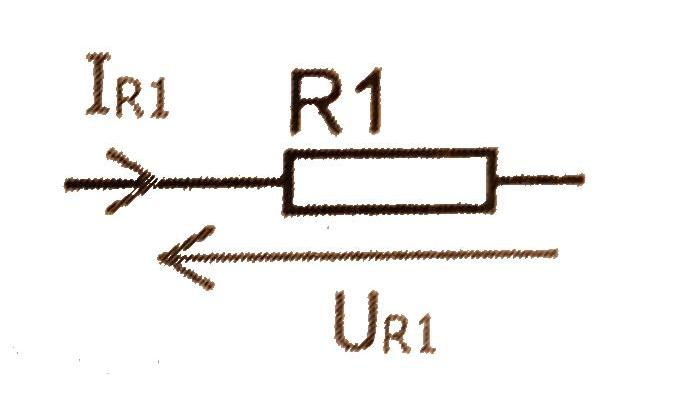
\includegraphics[scale = 0.15]{ohm}
 \end{center}
\end{figure}


\subsection{Loi des mailles, loi des noeuds}

\subsubsection{Loi des mailles}

Sur une maille (boucle), la somme algébrique des tensions est nulle.

Méthode d'utilisation de la loi des mailles : 
\begin{enumerate}
 \item prendre un point de départ quelconque (par exemple : A)
 \item tracer une maille (boucle) qui part au point A et y revient : flécher le sens de parcours de cette maille*
 \item flécher toutes les tensions de la maille.
 \item la somme algébrique des tensions formant cette maille est égale à zéro.
\end{enumerate}

\paragraph{Remarque :}
Dans cette somme, les tensions fléchées dans le même sens de parcours que la maille, sont comptées positivement et les autres négativement.

\paragraph{Exemple :}
Sur le schéma électrique suivant, on peut identifier 3 mailles partant du point A :

\begin{figure}[h]
 \begin{center}
  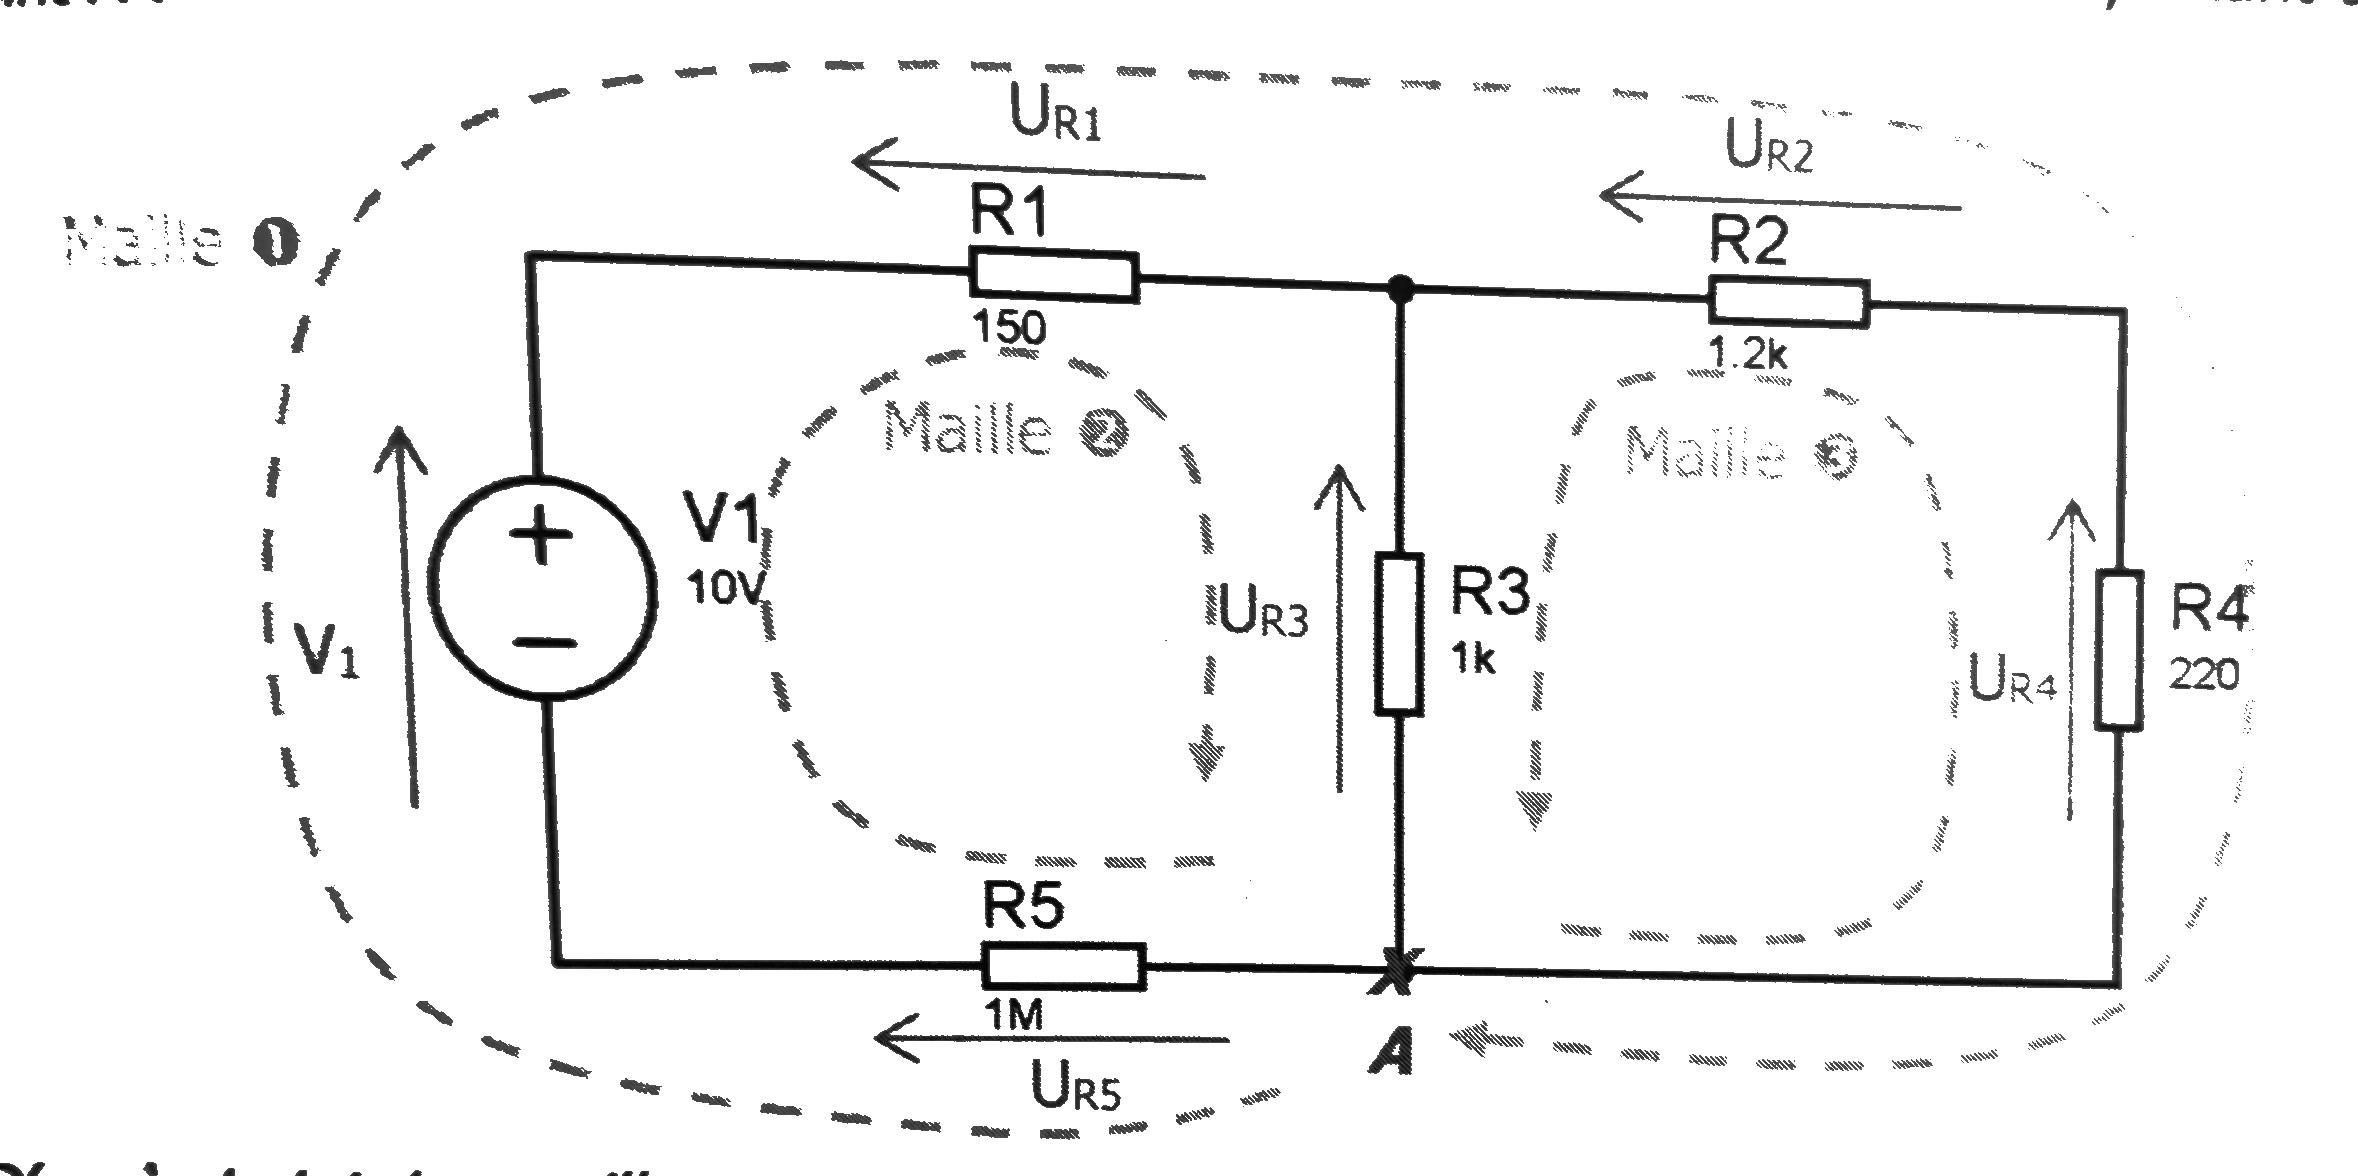
\includegraphics[width=\textwidth]{loidesmailles}
 \end{center}
\end{figure}

D'après la loi des mailles, on a :
\begin{itemize}
 \item Maille 1 : $U_{R5} + V_1 - U_{R1} - U_{R2} - U_{R4} = 0$
 \item Maille 2 : $U_{R5} + V_1 - U_{R1} - U_{R3} = 0$
 \item Maille 3 : $U_{R4} + U_{R2} - U_{R3} = 0$
\end{itemize}



\subsubsection{Loi des noeuds}
La somme des courants qui ``entrent'' dans un noeud électrique est égale à la somme des courants qui ``sortent'' de ce même noeud électrique :
$$\sum I_{entrant} = \sum I_{sortant}$$
\begin{figure}[h]
 \begin{center}
  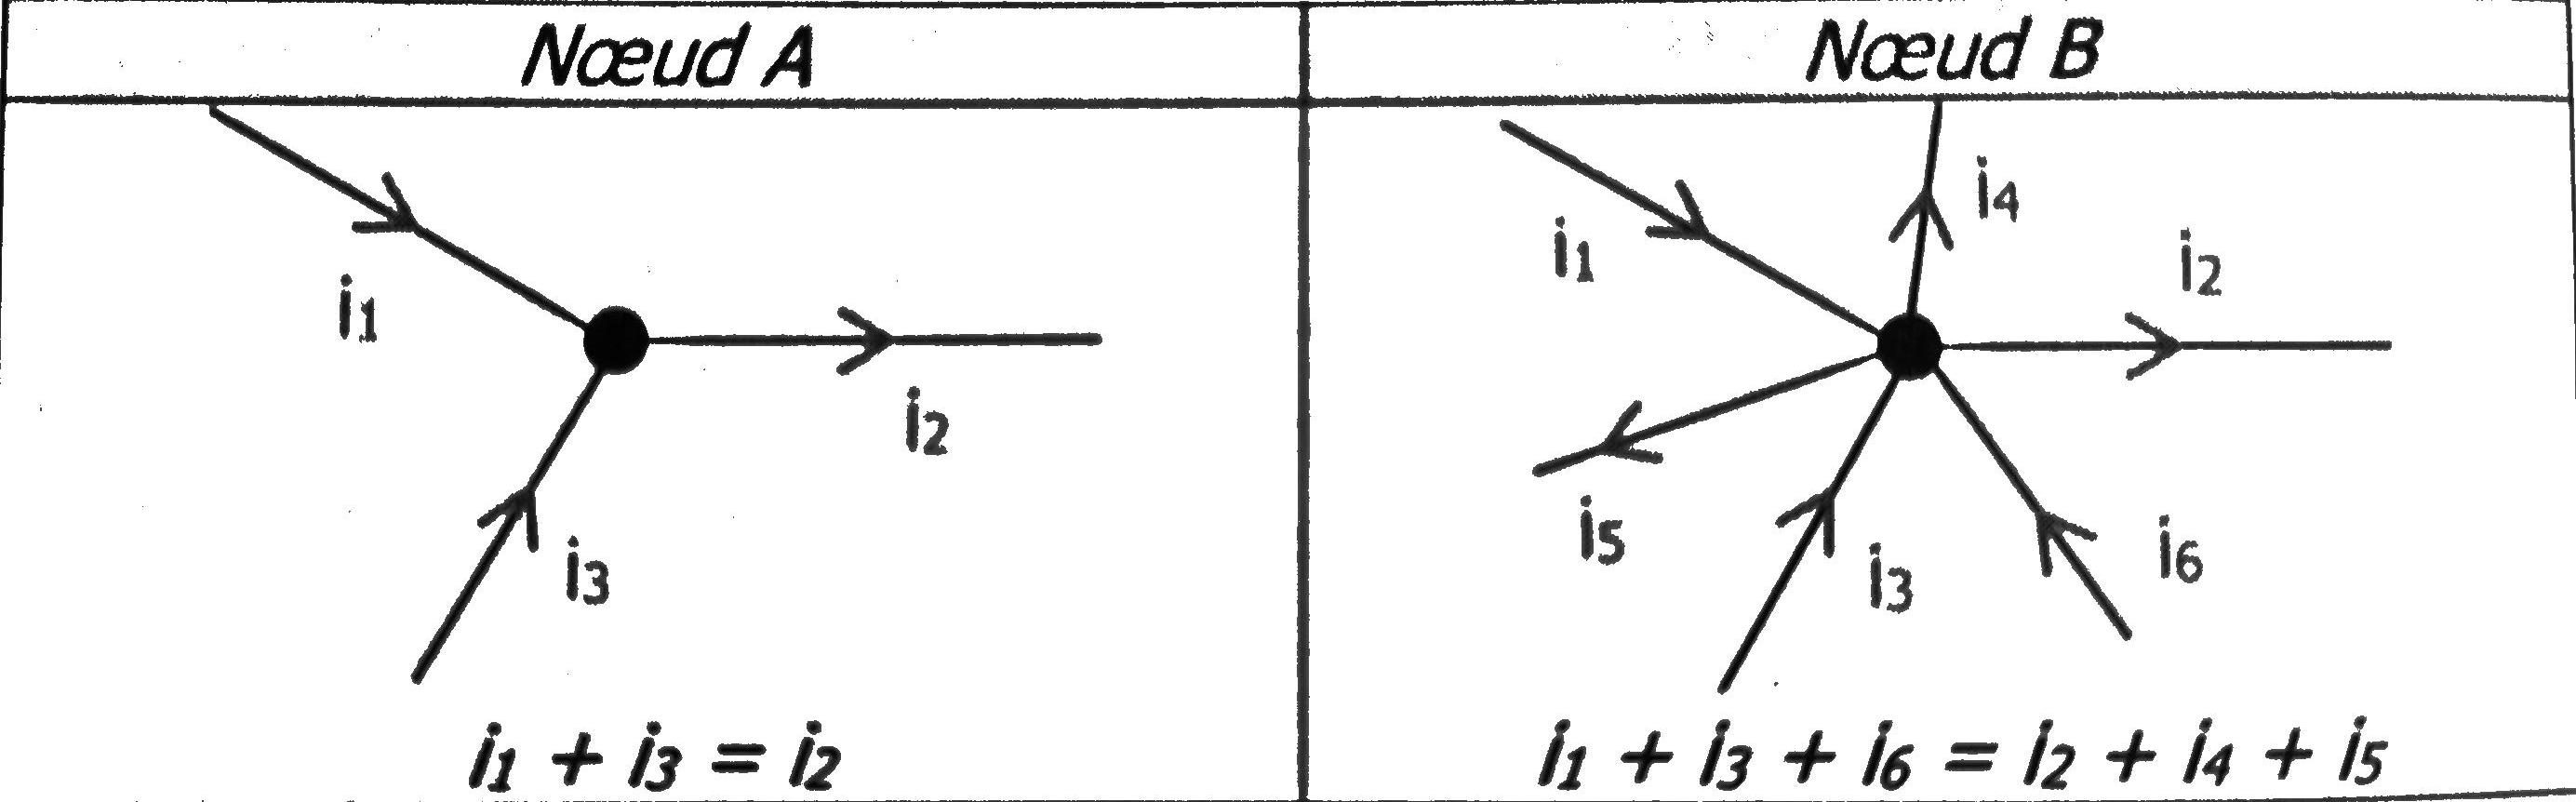
\includegraphics[width=\textwidth]{loisdesnoeuds}
 \end{center}
\end{figure}
\subsection{Théorème de superposition}
Le principe de superposition stipule que la tension à travers (ou le courant à travers) un élément dans un circuit linéaire est la somme algébrique des tensions à travers (ou des courants à travers) cet élément en raison de chaque source indépendante agissant seule.

\begin{figure}[h!]
 \begin{center}
  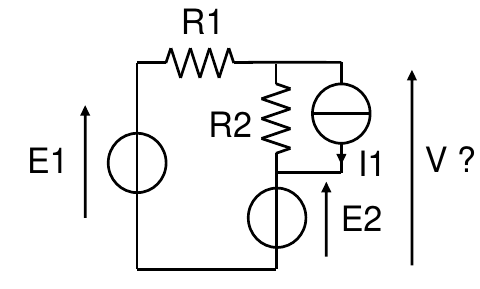
\includegraphics[scale=0.3]{superposition0}
  \caption{Schéma complet}
 \end{center}
\end{figure}

\begin{figure}[h!]
 \begin{center}
  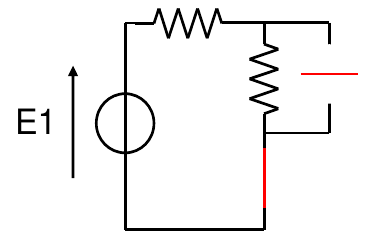
\includegraphics[scale=0.3]{superposition1}
  \caption{Schéma 1}
 \end{center}
\end{figure}

Ce qui nous donne : $$V_1=\frac{E_1\times R_2}{R_1+R_2}$$

\begin{figure}[h!]
 \begin{center}
  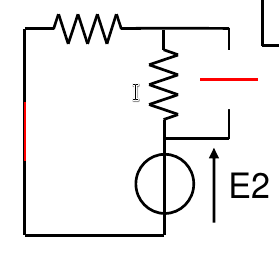
\includegraphics[scale=0.3]{superposition2}
  \caption{Schéma 2}
 \end{center}
\end{figure}

Ce qui nous donne : $$V_2=\frac{E_2\times R_1}{R_1+R_2}$$

\begin{figure}[h!]
 \begin{center}
  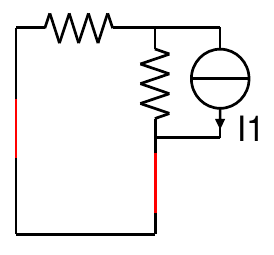
\includegraphics[scale=0.3]{superposition3}
  \caption{Schéma 3}
 \end{center}
\end{figure}

Ce qui nous donne : $$V_3=-I_1\times (R_1//R_2)$$

On a donc finalement : $$V = V_1 + V_2 + V_3$$
$$V = E_1\frac{R_2}{R_1+R_2}+E_2\frac{R_1}{R1+R2}-I1(R1//R2))$$

\subsection{Théorème de Millman}
Lorsqu'on a un montage électrique possédant plusieurs branches et qu'on souhaite connaître le potentiel du noeud central, on applique la relation : $$V_S = \frac{\sum \frac{potentiel}{resistance}}{\sum \frac{1}{resistance}}$$
\paragraph{Remarque :}
Le théorème du pont diviseur est un cas particulier du théorème de Millman.

\paragraph{Exemple :}
Application au montage ci-contre : $$V_S = \frac{\frac{V_1}{R_8}+\frac{V_2}{R_9}+\frac{V_3}{R_10}}{\frac{1}{R_8}+\frac{1}{R_9}+\frac{1}{R_10}}$$
\begin{figure}[h]
 \begin{center}
  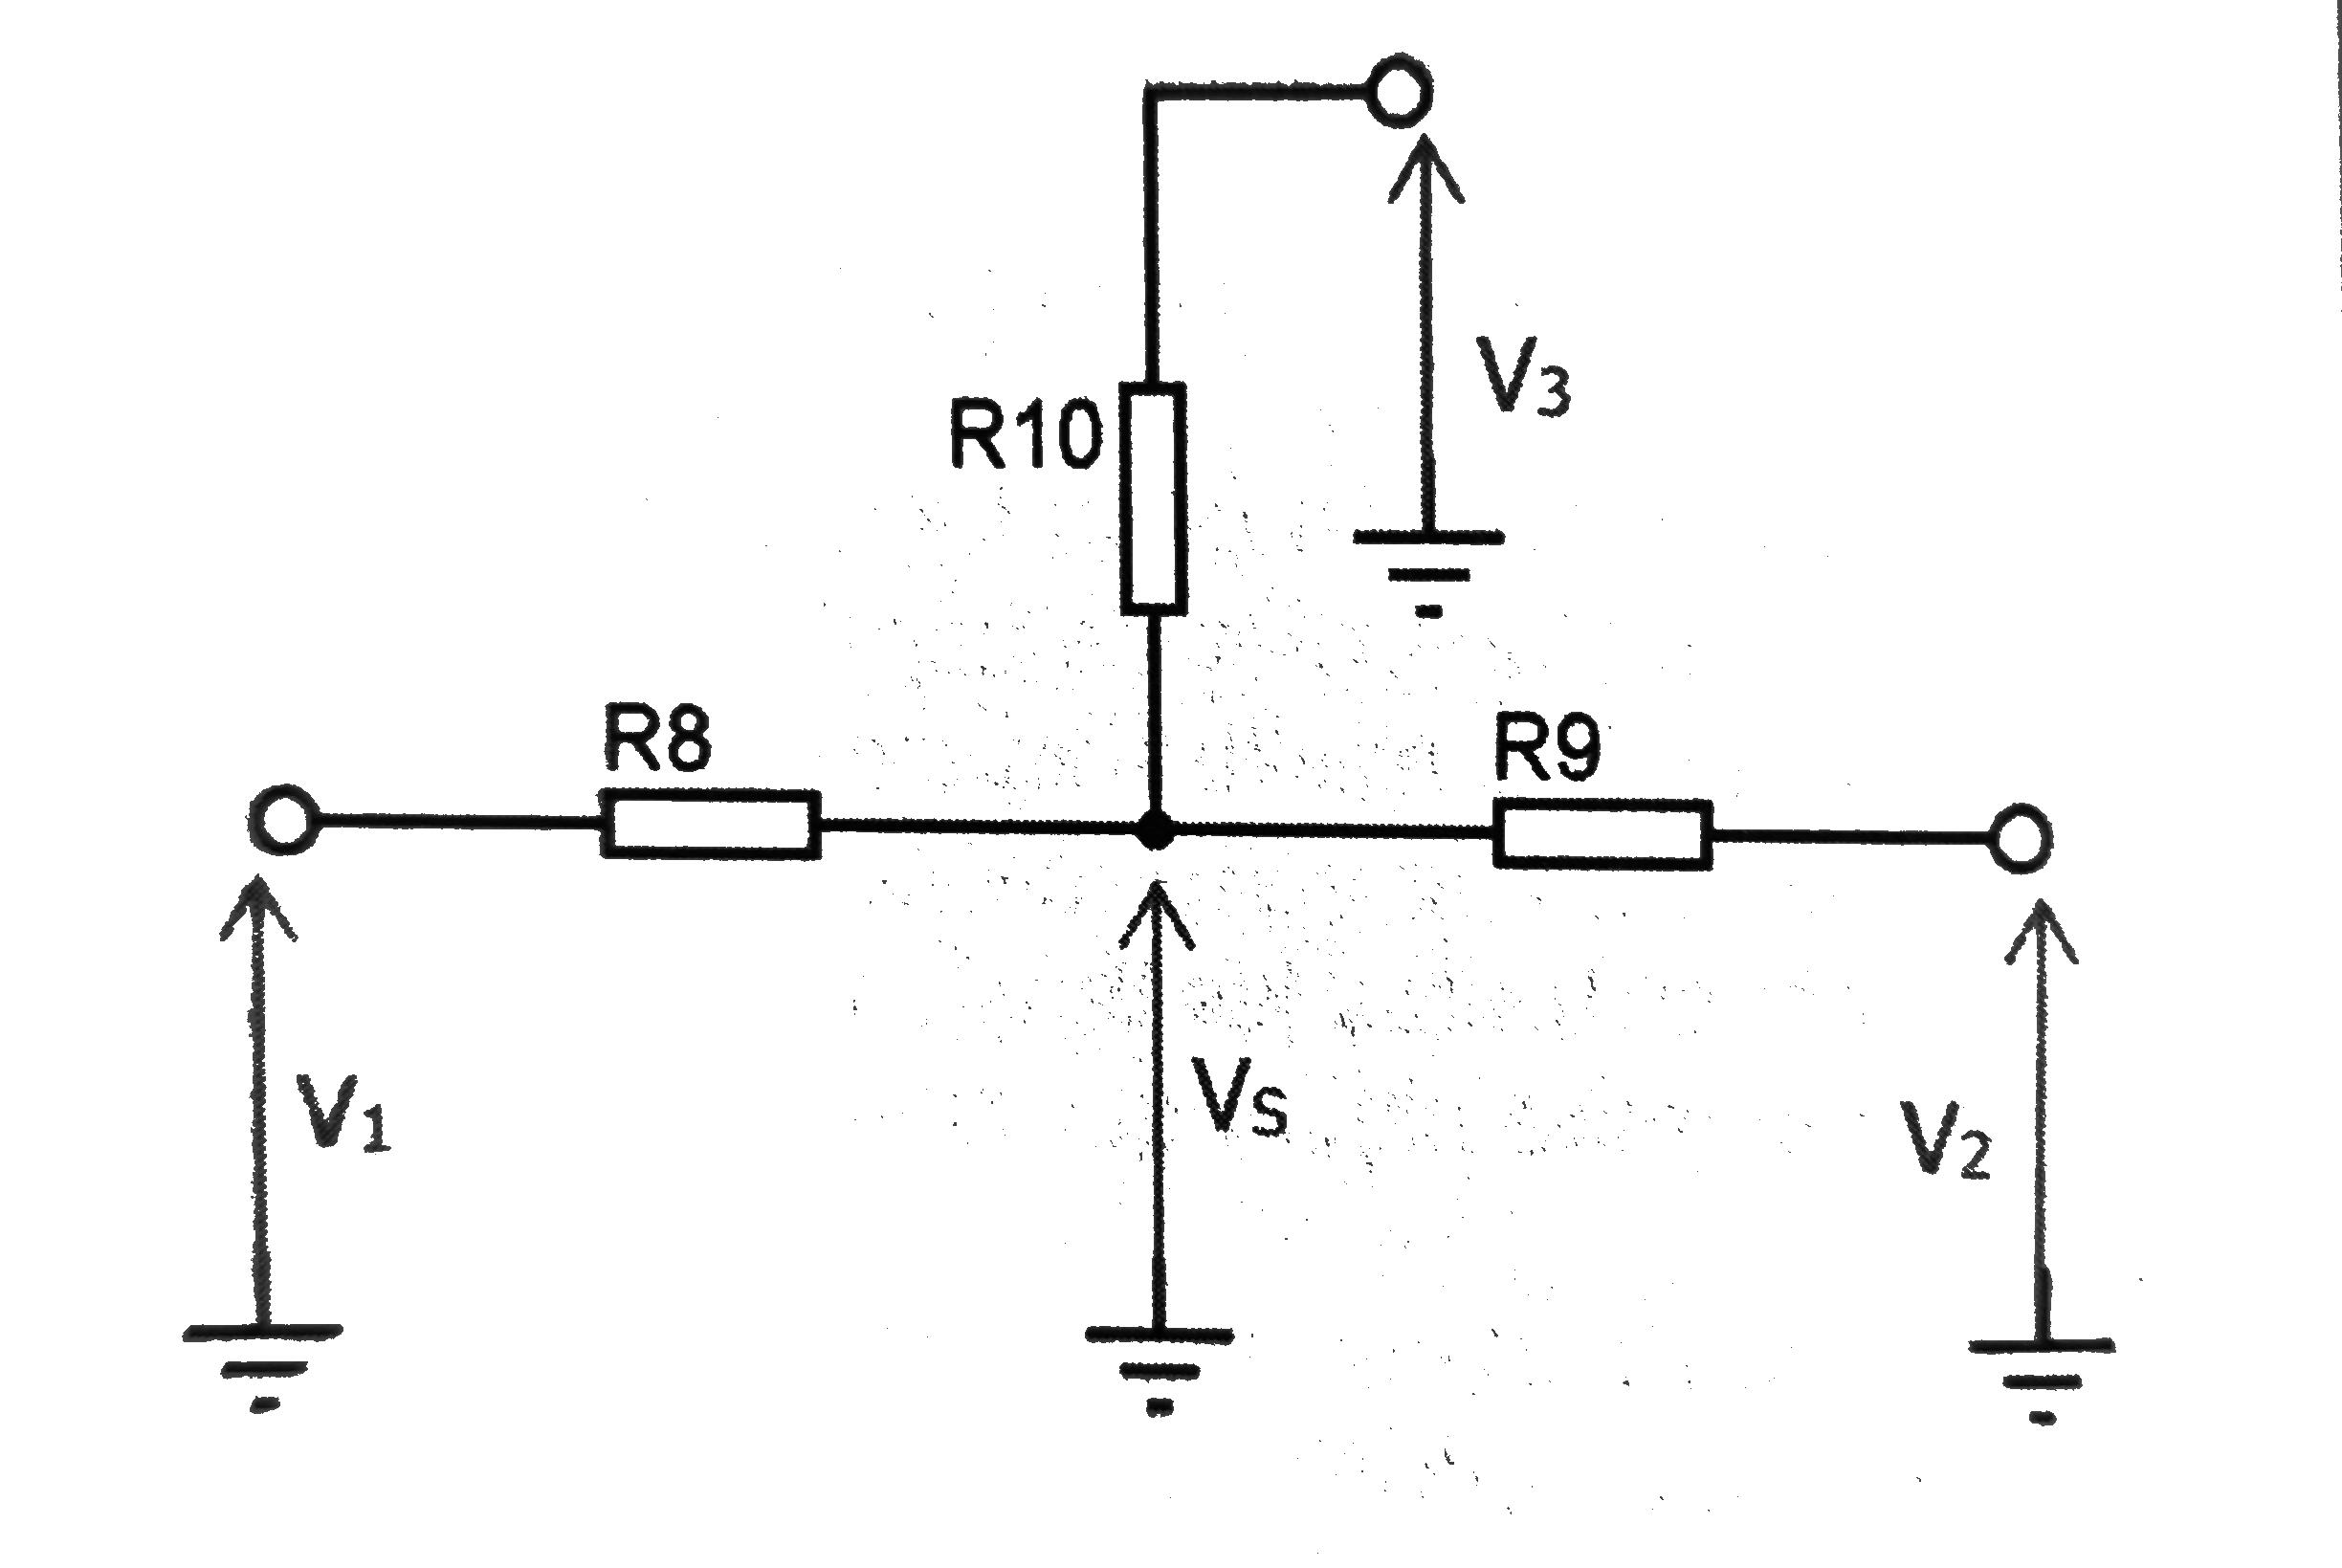
\includegraphics[width=\textwidth]{millman}
 \end{center}
\end{figure}
\subsection{Équivalences Thévénin-Norton}
Le modèle de Thévenin consiste en l’association série d’une source idéale de tension E avec
une résistance r. Il permet de décrire tous les dipôles actifs linéaires dont la caractéristique
courant-tension est un segment de droite.


\section{Régime Transitoire}
\subsection{Équations caractéristiques de la bobine et du condensateur}
\subsubsection{Le condensateur}
Si le courant est constant, la quantité d’électricité transportée pendant la durée $\Delta t$ est :
$$\Delta q = i \times \Delta t$$
Avec $\Delta q$ en Coulomb (C), $i$ en Ampère (A) et $\Delta t$ en seconde (s).

On charge le condensateur à l’aide d’un générateur de courant
constant et on relève la tension $u_{AB}$ et la charge $q$ à des
intervalles de temps réguliers.

Par conséquent, la caractéristique a pour équation : $q = C u_{AB}$ C représente la \textbf{capacité du condensateur} et s’exprime en
Farad (F)
$$i=C\frac{du}{dt}$$

Si la tension aux bornes du condensateur est variable, le courant dans le
condensateur est différent de zéro.

Si la tension aux bornes du condensateur est constante, c’est que sa charge
(ou décharge) est terminée.

\subsubsection{Énergie stockée par un condensateur}
$$\Delta E_{elec}=\frac{1}{2}UQ=\frac{1}{2}C\times U^2$$

\subsubsection{Association de condensateurs}

\paragraph{Association parallèle}

$$C_{eq}=C_1+C_2+...+C_n$$

\paragraph{Association série}

$$\frac{1}{C_{eq}}=\frac{1}{C_1}+\frac{1}{C_2}+...+\frac{1}{C_n}$$

\subsubsection{La bobine}

Une bobine est constituée par l’enroulement régulier d’un fil métallique
conducteur. Cette bobine peut être plate ou longue (solénoïde). Une bobine
n’a d’existence que si le courant est variable.

$$u=L\frac{di}{dt}$$

Unité : L’inductance d’une bobine s’exprime en Henry (H)

Une bobine ne peut subir de discontinuité de courant. Le
courant électrique dans un circuit inductif ne peut pas
s’interrompre instantanément.


Si le courant dans la bobine est constant, alors la tension à ses
bornes est nulle.

Il ne peut y avoir de tension que si le courant est variable.
Donc une bobine alimentée en courant continu se comporte
comme un court-circuit.

\subsubsection{Énergie d'une bobine}
L’énergie magnétique emmagasinée dans une bobine
d’inductance L, parcourue par un courant d’intensité I est :

$$E_{mag}=\frac{1}{2}LI^2$$ $E_{mag}$ en joule (J) ; $L$ en Henry (H) ; et $I$ en Ampère (A)

Une bobine idéale ne dissipe pas d’énergie ou de chaleur.
Elle ne fait que l’emmagasiner et la restituer.

\subsubsection{Association de bobines}

\paragraph{Association série}

$$L_{eq}=L_1+L_2+...+L_n$$


\paragraph{Association parallèle}

$$\frac{1}{L_{eq}}=\frac{1}{L_1}+\frac{1}{L_2}+...+\frac{1}{L_n}$$



\subsection{Comportement des circuits RC, RL et RLC}

\subsubsection{Circuit RC}
Ce circuit possède un générateur, une résistance et un condensateur.
\subsubsection{RL}
Ce circuit possède un générateur, une résistance et une bobine.
\subsubsection{RLC}
Ce circuit possède un générateur, une résistance, un condensateur et une bobine.
\end{document}
